\section{Implementación en CODESYS}

\begin{frame}{CODESYS: codificación manual (IEC 61131)}
  \begin{columns}[T]
    \begin{column}{0.58\textwidth}
      \begin{block}{De Stateflow/Simulink a un PLC}
        Los Niveles 0 y 1 se traducen a \textbf{SFC} (Sequential Function Charts) con cálculos en
        \textbf{ST} (Structured Text); el Nivel 2 se rehace con bloques de función de Matlab
        (\textit{simil ST}).
      \end{block}
      \begin{block}{Ejecución}
        Dos POUs principales (Niveles 0 y 1) cíclicos e independientes. En el PLC virtual
        (una sola CPU) se ejecutan secuencialmente intercalados, equivalente a paralelo.
      \end{block}
    \end{column}
    \begin{column}{0.42\textwidth}
      \centering
      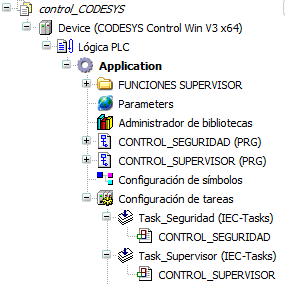
\includegraphics[width=0.85\linewidth]{codesys/arbol_codesys.png}\\
      \footnotesize Árbol de componentes del proyecto
    \end{column}
  \end{columns}
\end{frame}

\begin{frame}{Control regulatorio en simil ST: diagramas}
  Se rehace el Nivel 2 con la misma lógica pero con bloques de función de Matlab (simil ST);
  se agregan bloques \textit{Delay} para resolver loops algebraicos.
  \begin{figure}
    \centering
    \begin{subfigure}{0.49\textwidth}
      \centering
      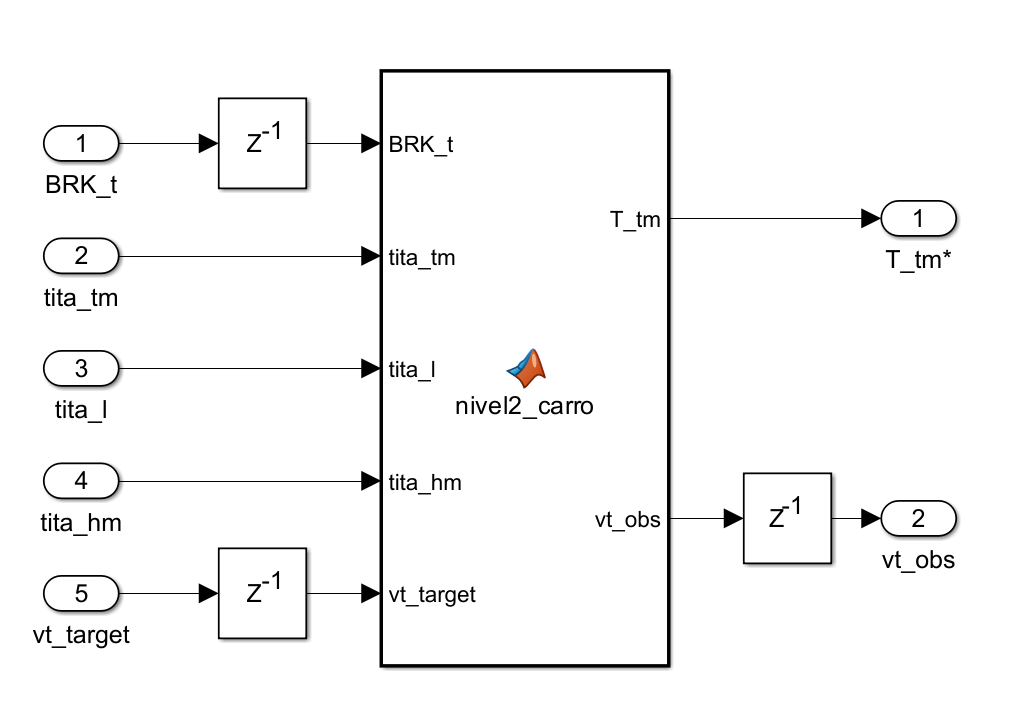
\includegraphics[width=\linewidth]{codesys/control_carro_funciones2.png}
      \caption{Control del carro}
    \end{subfigure}
    \hfill
    \begin{subfigure}{0.49\textwidth}
      \centering
      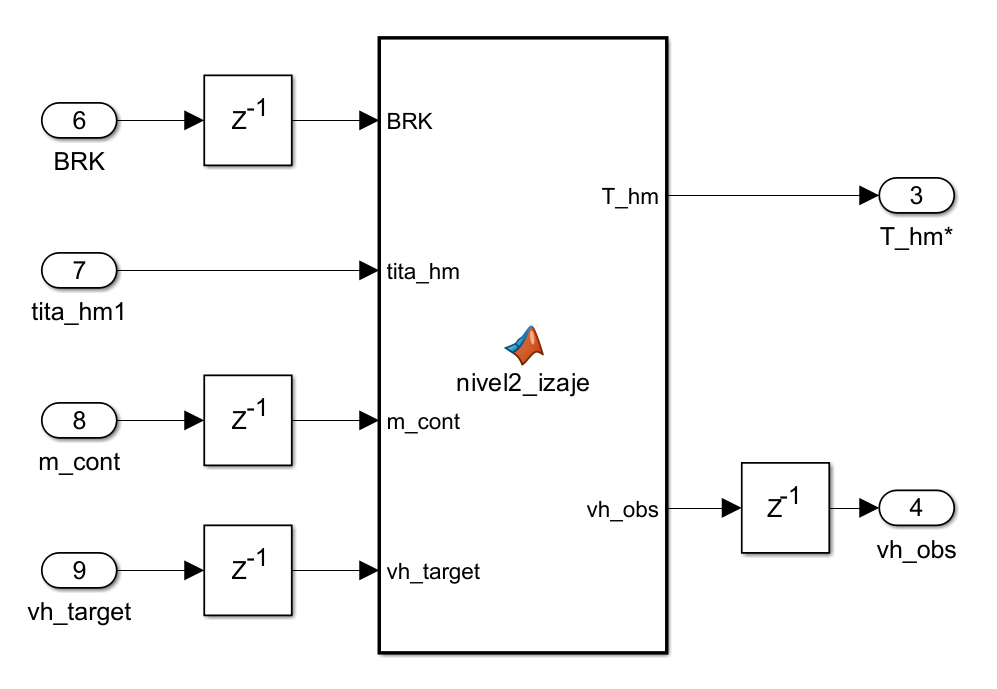
\includegraphics[width=\linewidth]{codesys/control_izaje_funciones2.png}
      \caption{Control del izaje}
    \end{subfigure}
  \end{figure}
\end{frame}

\begin{frame}{Control regulatorio en simil ST: código}
  El código de cada controlador (dentro de cada bloque de función de Matlab):
  \begin{figure}
    \centering
    \begin{subfigure}{0.42\textwidth}
      \centering
      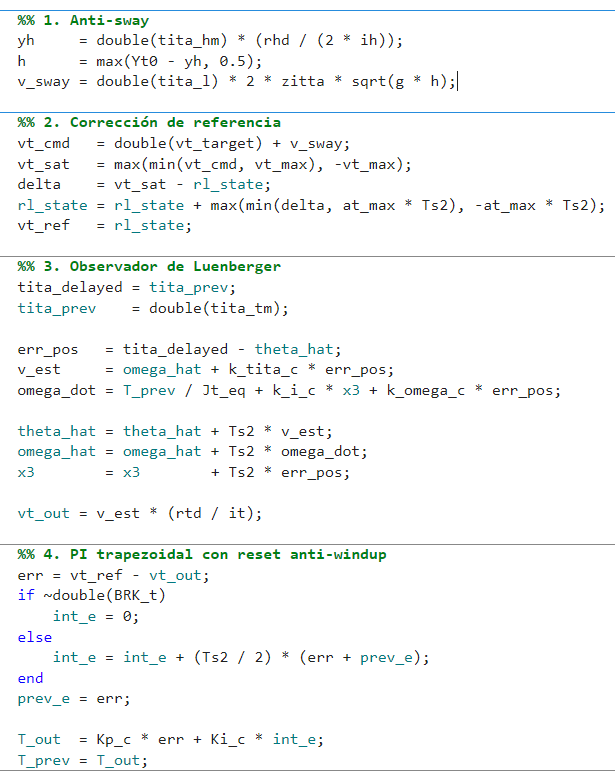
\includegraphics[width=\linewidth]{codesys/matlab_function_nivel2_carro.png}
      \caption{Control del carro (simil ST)}
    \end{subfigure}
    \hfill
    \begin{subfigure}{0.42\textwidth}
      \centering
      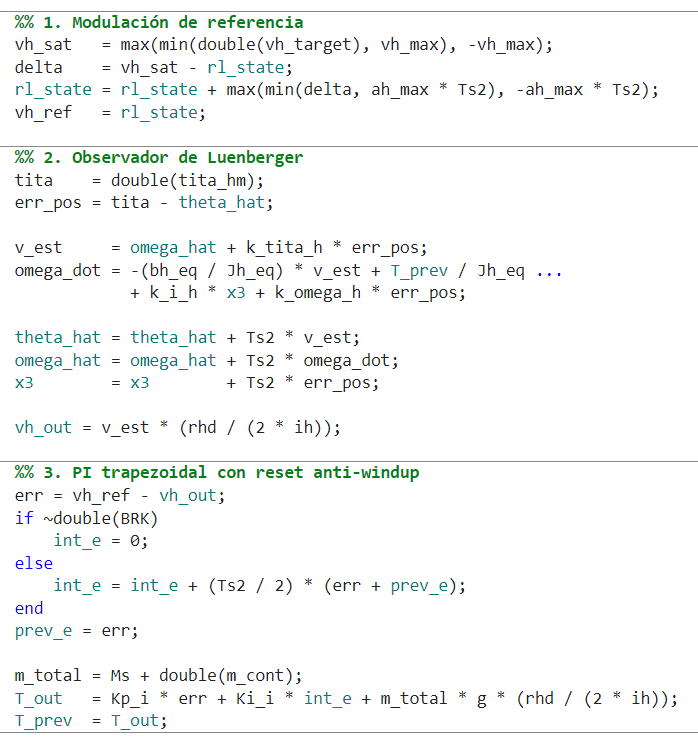
\includegraphics[width=\linewidth]{codesys/matlab_function_nivel2_izaje.png}
      \caption{Control del izaje (simil ST)}
    \end{subfigure}
  \end{figure}
\end{frame}
